%!TEX encoding = UTF-8 Unicode

\documentclass[a4paper]{article}

\usepackage{INTERSPEECH_v2}

\usepackage[T1]{fontenc} % output - specifies encoding used in fonts; needs full LaTeX distribution to produce good-looking output
\usepackage[utf8]{inputenc} % input - type accented characters directly from keyboard
\usepackage[english]{babel} % internationalization - hyphenation, typographic rules for one or more languages

\usepackage[nolist]{acronym}
\usepackage{amsmath}
\usepackage{amssymb}
%\usepackage{epigraph}
\usepackage{hyperref}
\graphicspath{{figures/}}

\title{Interactive Robot Learning of Gestures, Language and Affordances}
\name{Giovanni~Saponaro$^1$, Giampiero~Salvi$^2$, Lorenzo~Jamone$^{3,1}$, Alexandre~Bernardino$^1$}
\address{
  $^1$Institute for Systems and Robotics\\Instituto Superior Técnico, Universidade de Lisboa, Lisbon, Portugal\\
  $^2$KTH Royal Institute of Technology, Stockholm, Sweden\\
  $^3$ARQ~(Advanced Robotics at Queen Mary)\\School of Electronic Engineering and Computer Science, Queen Mary University of London, UK}
\email{gsaponaro@isr.tecnico.ulisboa.pt, giampi@kth.se, l.jamone@qmul.ac.uk, alex@isr.tecnico.ulisboa.pt}

% custom commands and frequent expressions that require typesetting care
\newcommand{\eg}{e.\,g.}
\newcommand{\ie}{i.\,e.}
\newcommand{\HR}{Human--Robot}
\newcommand{\HRI}{\HR{} Interaction}
\newcommand{\hh}{human--human}
\newcommand{\hr}{human--robot}
\newcommand{\hri}{\hr{} interaction}

\newcommand{\phmm}{\ensuremath{p_{\mbox{\scriptsize HMM}}}}
\newcommand{\pbn}{\ensuremath{p_{\mbox{\scriptsize BN}}}}

% examples and useful stuff from INTERSPEECH template

% \begin{table}
%   \caption{This is an example of a table}
%   \label{tab:example}
%   \centering
%   \begin{tabular}{ r@{}l  r }
%     \toprule
%     \multicolumn{2}{c}{\textbf{Ratio}} &
%                                          \multicolumn{1}{c}{\textbf{Decibels}} \\
%     \midrule
%     $1$                       & $/10$ & $-20$~~~             \\
%     $1$                       & $/1$  & $0$~~~               \\
%     $2$                       & $/1$  & $\approx 6$~~~       \\
%     $3.16$                    & $/1$  & $10$~~~              \\
%     $10$                      & $/1$  & $20$~~~              \\
%     $100$                     & $/1$  & $40$~~~              \\
%     $1000$                    & $/1$  & $60$~~~              \\
%     \bottomrule
%   \end{tabular}
% \end{table}

%\begin{figure}
%  \centering
%  \includegraphics[width=\linewidth]{figure.pdf}
%  \caption{Schematic diagram of speech production.}
%  \label{fig:speech_production}
%\end{figure}

% For technical reasons, the proceedings editor will strip all active links from the papers during processing. Hyperlinks can be included in your paper, if written in full, e.\,g.\ ``http://www.foo.com/index.html''. The link text must be all black.
% Please make sure that they present no problems in printing to paper.

% list of acronyms
\begin{acronym}
\acro{BN}{Bayesian Network}
\acro{HMM}{Hidden Markov Model}
\acro{MTRNN}{Multiple Timescales Recurrent Neural Network}
\end{acronym}

\begin{document}

\maketitle
%
\begin{abstract} % max 200 words
  place holder place holder place holder place holder place holder place holder place holder
  place holder place holder place holder place holder place holder place holder place holder
  place holder place holder place holder place holder place holder place holder place holder
  place holder place holder place holder place holder place holder place holder place holder

  place holder place holder place holder place holder place holder place holder place holder
  place holder place holder place holder place holder place holder place holder place holder
  place holder place holder place holder place holder place holder place holder place holder
  place holder place holder place holder place holder place holder place holder place holder
  place holder place holder place holder place holder place holder place holder place holder
  place holder place holder place holder place holder place holder place holder place holder
\end{abstract}
\noindent\textbf{Index Terms}: cognitive robotics, gesture recognition, object affordances

%%%%%%%%%%%%%%%%%%%%%%%%%%%%%%%%%%%%%%%%%%%%%%%%%%%%%%%%%%%%%%%%%%%%%%%%%%%%%%%%
%!TEX encoding = UTF-8 Unicode

\section{Introduction}

Robotics is progressing fast, with a steady and systematic shift from the industrial domain to domestic, public and leisure environments~\cite[ch.~65, Domestic Robotics]{siciliano:2016:handbook2}. Application areas that are particularly relevant and being researched by the scientific community include: robots for people's health and active aging, mobility, advanced manufacturing~(Industry~4.0). In short, all domains that require direct and effective \hri{} and communication (including language and gestures~\cite{matuszek:2014:aaai}).

However, robots have not reached the level of performance that would enable them to work with humans in routine activities in a flexible and adaptive way, for example in the presence of sensor noise, or unexpected events not previously seen during the training or learning phase. One of the reasons to explain this performance gap between \hh{} teamwork and a \hr{} teamwork is in the collaboration aspect, \ie, whether the members of a team understand one another. Humans have the ability of working successfully in groups. They can agree on common goals~(\eg, through verbal and non-verbal communication), work towards the execution of these goals in a coordinated way, and understand each other's physical actions~(\eg, body gestures) towards the realization of the final target. Human team coordination and mutual understanding is effective~\cite{ramnani:2004:natureneuro} because of~(i) the capacity to \emph{adapt} to unforeseen events in the environment, and re-plan one's actions in real time if necessary, and~(ii) a common motor repertoire and action model, which permits us to understand a partner's physical actions and manifested intentions as if they were our own~\cite{saponaro:2013:crhri}.

In neuroscience research, visuomotor neurons~(\ie, neurons that are activated by visual stimuli) have been a subject of ample study~\cite{rizzolatti:2001:nrn}. Mirror neurons are one class of such neurons that responds to action and object interaction, both when the agent acts and when it observes the same action performed by others, hence the name ``mirror''.

\begin{figure}
  \centering
  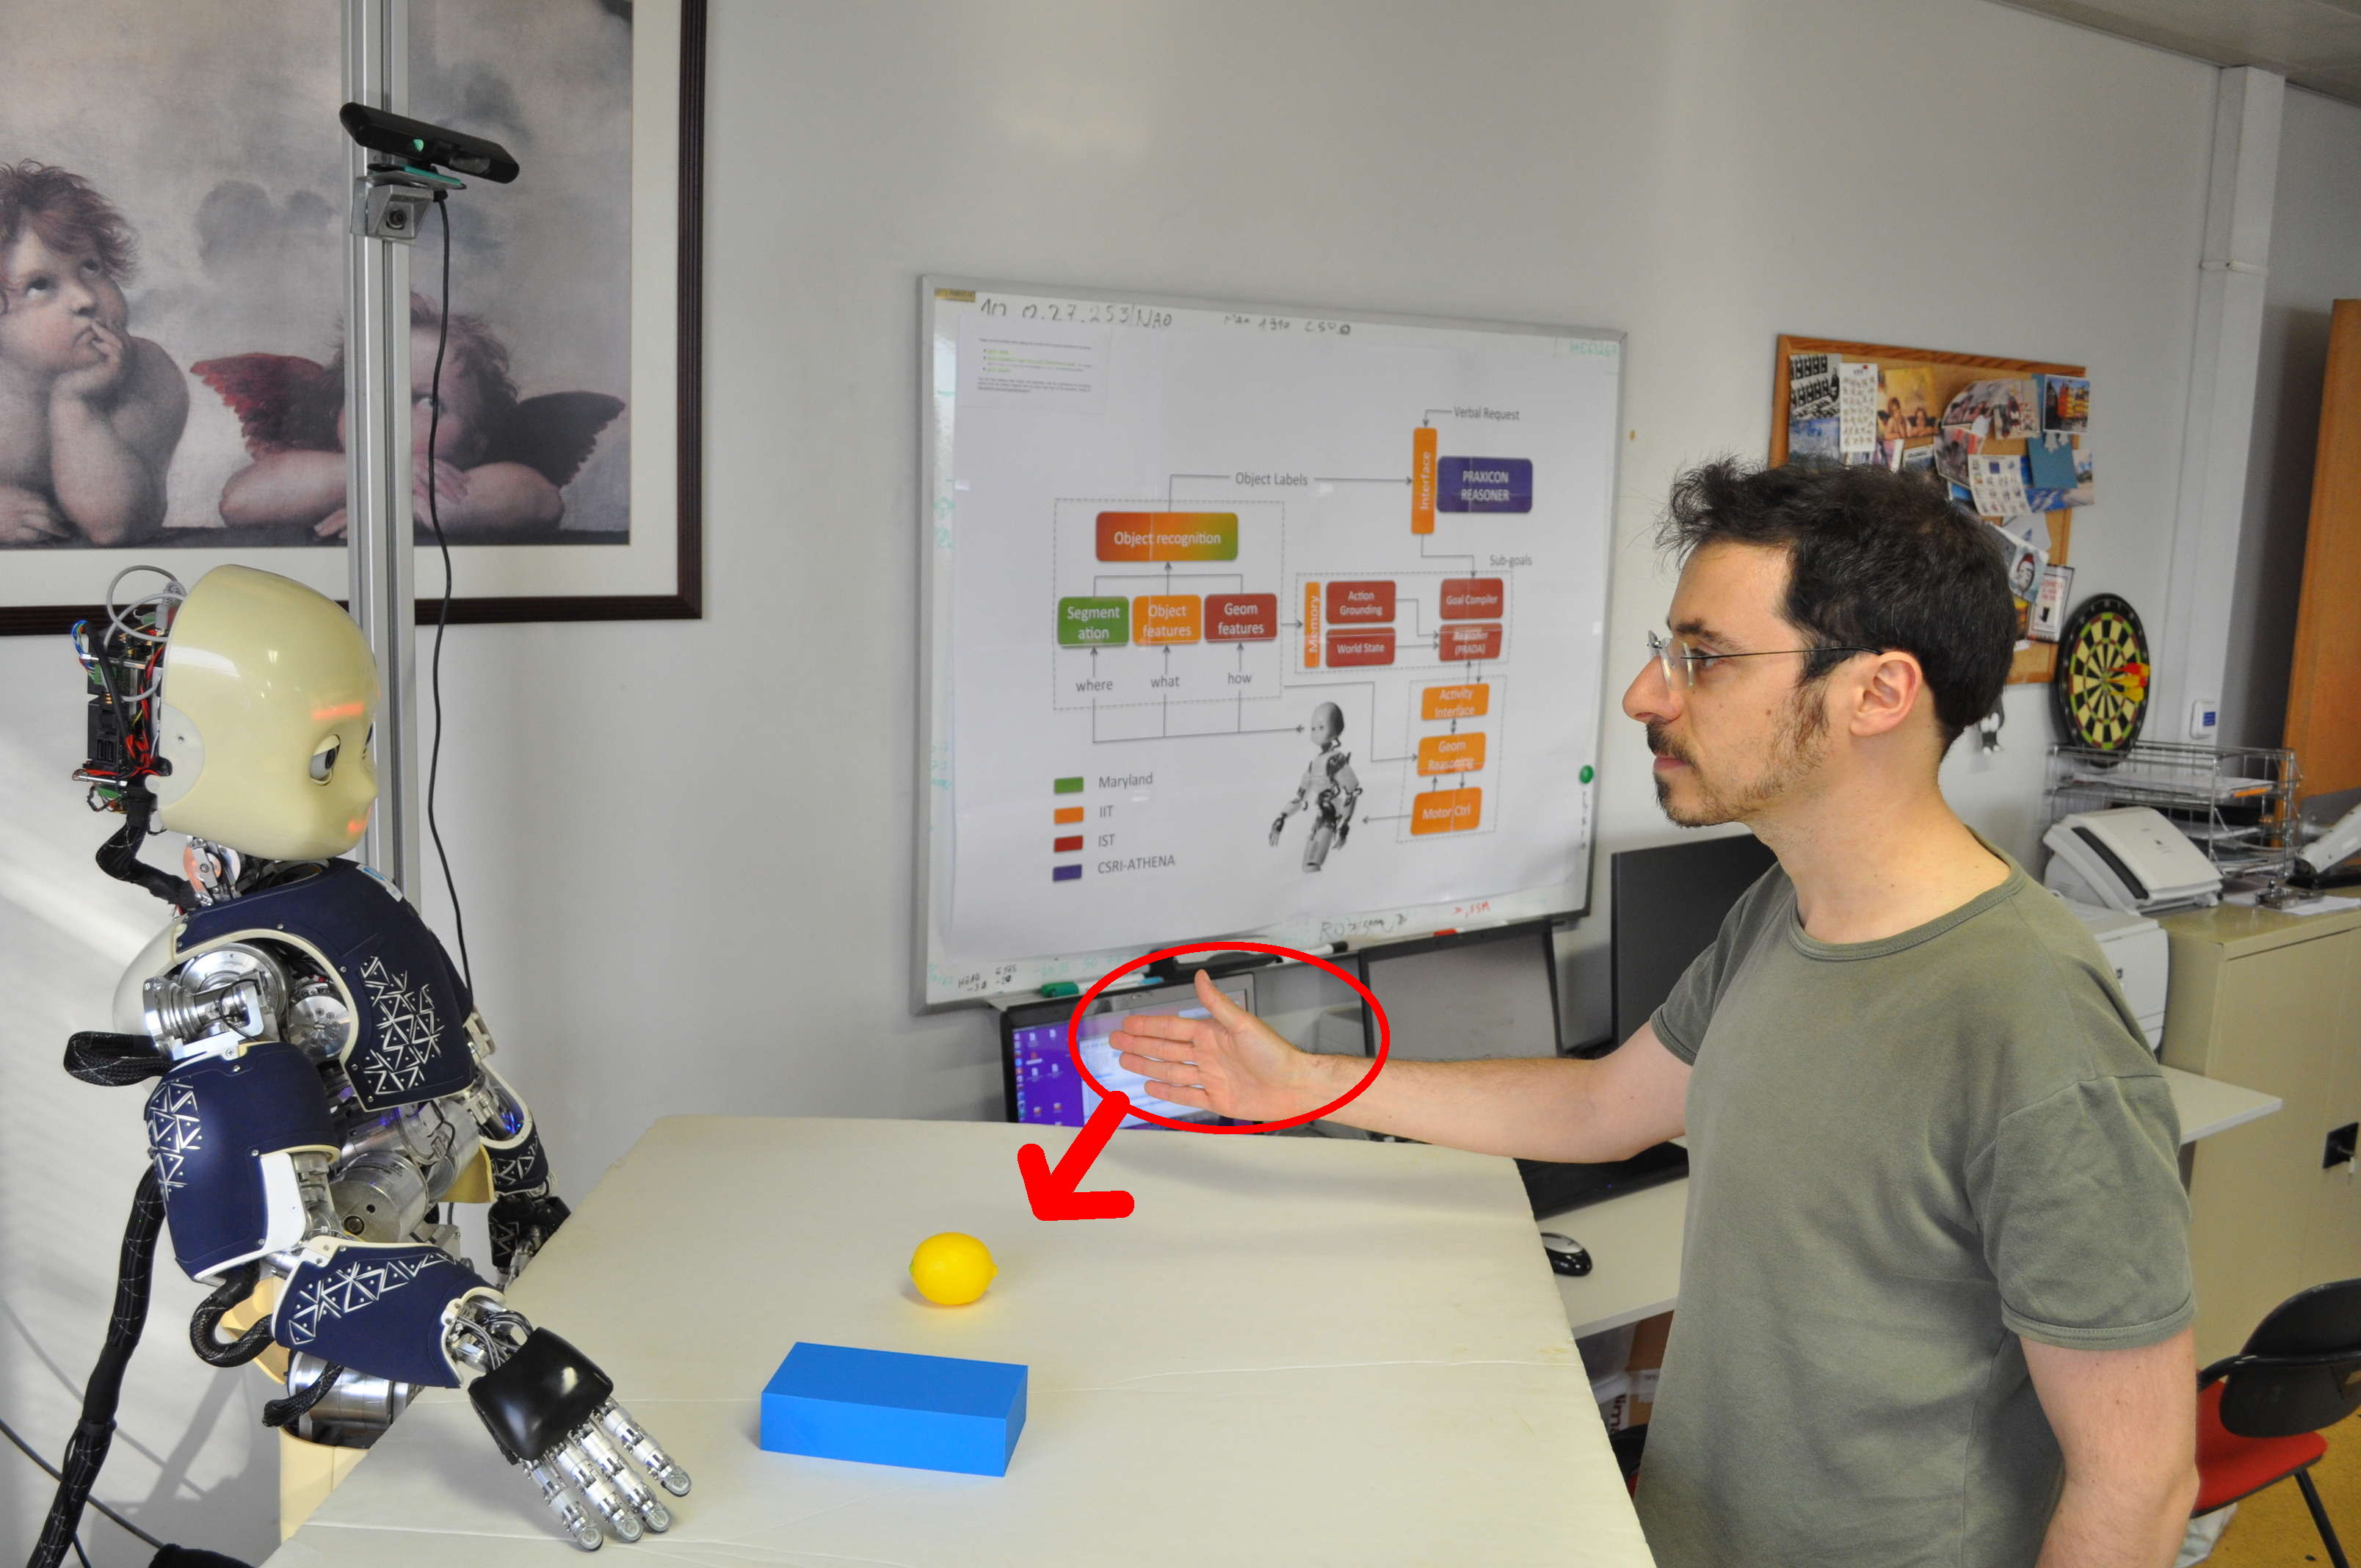
\includegraphics[width=0.9\columnwidth]{human_tap}
  \caption{Experimental setup, consisting of an iCub humanoid robot and a human user performing a manipulation gesture on a shared table with different objects on top. The depth sensor in the top-left corner is used to extract human hand coordinates for gesture recognition. Depending on the gesture and on the target object, the resulting effect will differ.}
  \label{fig:experimental_setup}
\end{figure}

This work takes inspiration from the theory of mirror neurons, and contributes towards using it on humanoid and cognitive robots. We show that a robot can first acquire knowledge by sensing and self-exploring its surrounding environment~(\eg, by interacting with available objects and building up an affordance representation of the interactions and their outcomes) and, as a result, the robot is capable of generalizing its acquired knowledge while observing another agent~(\eg, a human person) who performs similar physical actions to the ones executed during prior robot training. Fig.~\ref{fig:experimental_setup} shows the experimental setup.


%%%%%%%%%%%%%%%%%%%%%%%%%%%%%%%%%%%%%%%%%%%%%%%%%%%%%%%%%%%%%%%%%%%%%%%%%%%%%%%%
%!TEX encoding = UTF-8 Unicode

\section{Related Work}

A large and growing body of research is directed towards having robots learn new cognitive skills, or improving their capabilities, by interacting autonomously with their surrounding environment. In particular, robots operating in an unstructured scenario may understand available opportunities conditioned on their body, perception and sensorimotor experiences: the intersection of these elements gives rise to object affordances~(action possibilities), as they are called in psychology~\cite{gibson:2014}. The usefulness of affordances in cognitive robotics is in the fact that they capture essential properties of environment objects in terms of the actions that a robot is able to perform with them~\cite{montesano:2008,jamone:2016:tcds}.
Some authors have suggested an alternative computational model called \acp{OAC}~\cite{kruger:2011:ras}, which links low-level sensorimotor knowledge with high-level symbolic reasoning hierarchically in autonomous robots.

In addition, several works have demonstrated how combining robot affordance learning with language grounding can provide cognitive robots with new and useful skills, such as learning the association of spoken words with sensorimotor experience~\cite{salvi:2012:smcb,morse:2016:cogsci} or sensorimotor representations~\cite{stramandinoli:2016:icdl}, learning tool use capabilities~\cite{goncalves:2014:icarsc,goncalves:2014:icdl}, and carrying out complex manipulation tasks expressed in natural language instructions which require planning and reasoning~\cite{antunes:2016:icra}.

% Here you can specify that the fact that the action is known a priori is used during training of the model
% the model can be then used to infer the action as well, but based on the evidence from the other nodes.
% In the current study, in contrast:
% 1) we want to infer the action from the HMMs during training
% 2) during testing we may merge the infromation from the HMMs with that from the Bayesian Network.
In~\cite{salvi:2012:smcb}, a joint model to learn robot affordances~(\ie, relationships between actions, objects and resulting effects) together with word meanings is proposed. That framework assumes that the robot action is known a~priori during the training phase~(\eg, the information ``grasping'' during a grasping experiment is given), and the resulting model can be used at testing to make inferences about the environment, including estimating the most likely action, based on evidence from other pieces of information.

Several neuroscience and psychology studies build upon the theory of mirror neurons which we brought up in the Introduction. These studies indicate that perceptual input can be linked with the human action system for predicting future outcomes of actions, \ie, the effect of actions, particularly when the person possesses concrete personal experience of the actions being observed in others~\cite{aglioti:2008:basketball,knoblich:2001:psychsci}. This has also been exploited under the deep learning paradigm~\cite{kim:2017:nn}, by using a \ac{MTRNN} to have an artificial simulated agent infer human intention from joint information about object affordances and human actions. One difference between this line of research and ours is that we use real, noisy data acquired from robots and sensors to test our models, rather than virtual simulations.


%%%%%%%%%%%%%%%%%%%%%%%%%%%%%%%%%%%%%%%%%%%%%%%%%%%%%%%%%%%%%%%%%%%%%%%%%%%%%%%%
%!TEX encoding = UTF-8 Unicode

\section{Proposed Approach}

In this paper, we combine (1)~the robot affordance model of~\cite{salvi:2012:smcb}, which associates verbal descriptions to the physical interactions of an agent with the environment, with (2)~the gesture recognition system of~\cite{saponaro:2013:crhri}, which infers the type of action from human user movements. We consider three manipulation actions performed by agent(s) onto objects on a table~(see Fig.~\ref{fig:experimental_setup}): grasp, tap, and touch. We reason on the effects of these actions onto the objects of the world, and on the co-occurring verbal description of the experiments.

% TODO kinematic compatibility? (Lor)

Our main contribution is that of extending~\cite{salvi:2012:smcb} by relaxing the known-action assumption. We estimate the action performed by a human user during a \hr{} collaborative task, by employing statistical inference methods and \acp{HMM}. This provides two advantages. First, we can infer the executed action during training. Secondly, at testing time we can merge the action information obtained from gesture recognition with the information about affordances.

\begin{figure}
  \centering
  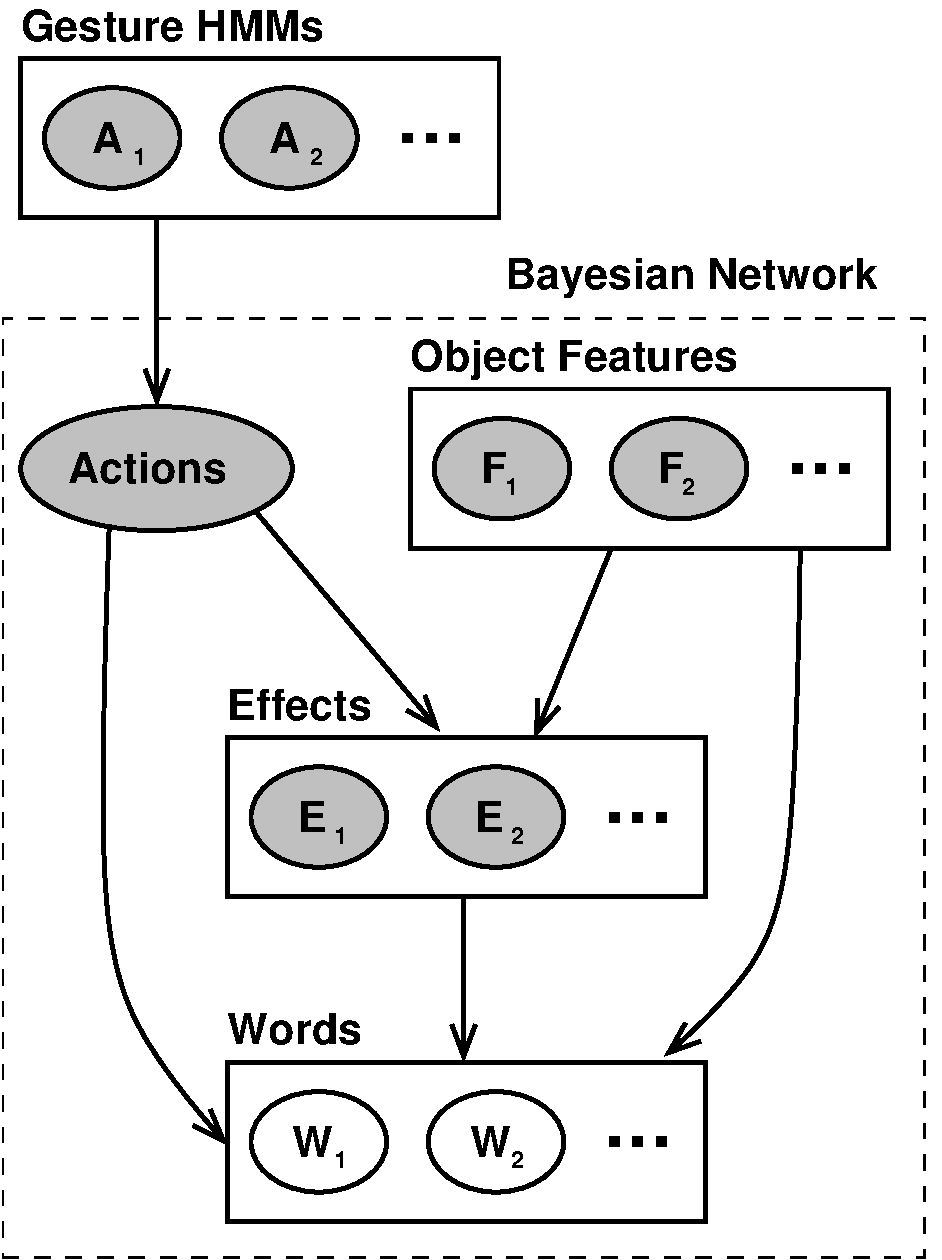
\includegraphics[width=0.8\columnwidth]{fullNetAbstract}
  \caption{Abstract representation of the probabilistic dependencies in the model. Shaded nodes are observable or measurable in the present study, and edges indicate Bayesian dependency.}
  \label{fig:model}
\end{figure}

\subsection{\acl{BN} for \AffWords{} Modeling}
\label{sec:bn}

Following the method adopted in~\cite{salvi:2012:smcb}, we use a Bayesian probabilistic framework to allow a robot to ground the basic world behavior and verbal descriptions associated to it. The world behavior is defined by random variables describing: the actions~$A$, defined over the set~$\mathcal{A} = \{a_i\}$, object properties~$F$, over $\mathcal{F} = \{f_i\}$, and effects~$E$, over~$\mathcal{E} = \{e_i\}$. We denote~$X = \{A, F, E\}$ the state of the world as experienced by the robot. The verbal descriptions are denoted by the set of words~$W = \{w_i\}$. Consequently, the relationships between words and concepts are expressed by the joint probability distribution~$p(X,W)$ of actions, object features, effects, and words in the spoken utterance. The symbolic variables and their discrete values are listed in Table~\ref{tab:bnsymb}.

\begin{table}
    \centering
    \caption{The symbolic variables of the \acl{BN} which we use in this work~(a subset of the ones from~\cite{salvi:2012:smcb}), with the corresponding discrete values obtained from clustering during previous robot exploration of the environment. In addition, our full model also includes word variables~(see Fig.~\ref{fig:model}), whose values are the probabilities of the words co-occurring in the associated verbal description of an experiment - PUT THIS LAST PHRASE AS FOOTNOTE?.}
    \label{tab:bnsymb}
    \begin{tabular}{*{3}{l}} % left-aligned columns
    \toprule
    name   & description     & values \\
    \midrule
    Action & action          & grasp, tap, touch \\
    Shape  & object shape    & sphere, box \\
    Size   & object size     & small, medium, big \\
    ObjVel & object velocity & slow, medium, fast \\
    \bottomrule
    \end{tabular}
\end{table}

This joint probability distribution, that is illustrated by the part of Fig.~\ref{fig:model} enclosed in the dashed box, is estimated by the robot in an ego-centric way through interaction with the environment, as in~\cite{salvi:2012:smcb}. As a consequence, during learning, the robot knows what action it is performing with certainty, and the variable~$A$ assumes a deterministic value. This assumption is relaxed in the present study, by extending the model to the observation of external~(human) agents as explained below.

\subsection{\aclp{HMM} for Gesture Recognition}

\newcommand{\myscalefactor}{0.8}

\newcommand{\standardhmm}[1]{
    \node[draw,circle] (hmm#1s1) {1};
    \node[draw,circle, right of=hmm#1s1] (hmm#1s2) {2};
    \node[circle, right of=hmm#1s2] (hmm#1s3) {\dots};
    \node[draw,circle, right of=hmm#1s3] (hmm#1s4) {Q};
    \node[left of=hmm#1s1]  (invisible1) {};
    \node[right of=hmm#1s4] (invisible2) {};
    \path[->] (hmm#1s1) edge (hmm#1s2);
    \path[loop above] (hmm#1s1) edge (hmm#1s1);
    \path[->] (hmm#1s2) edge (hmm#1s3);
    \path[loop above] (hmm#1s2) edge (hmm#1s2);
    \path[dashed] (hmm#1s2) -- (hmm#1s3);
    \path[->] (hmm#1s3) edge (hmm#1s4);
    \path[loop above] (hmm#1s4) edge (hmm#1s4);
    %\path[->] (hmm#1s4) edge[bend left] (hmm#1s1);
    \path[->] (invisible1) edge (hmm#1s1);
    \path[->] (hmm#1s4) edge (invisible2);
}

\newcommand{\modeltwo}{
  \begin{tikzpicture}[scale=\myscalefactor, every node/.style={scale=\myscalefactor}]
  \matrix (M) [matrix of nodes, ampersand replacement=\&] {%
    grasp gesture HMM \& \standardhmm{1} \\
    tap gesture HMM \& \standardhmm{2} \\
    touch gesture HMM \& \standardhmm{3} \\
    %garbage \& \standardhmm{4} \\
  };
  \end{tikzpicture}
}

\begin{figure}
  \centering
  \modeltwo
  \caption{Structure of the \acp{HMM} used for human gesture recognition, adapted from in~\cite{saponaro:2013:crhri}. In this work, we consider three independent, multiple-state \acp{HMM}, each of them trained to recognize one of the considered manipulation gestures. At test time, we can obtain likelihood scores of a new gesture being classified, \eg, $p(\text{grasp})=0.6, p(\text{tap})=0.3, p(\text{touch})=0.1$. Then we can either keep the probabilistic information~(soft decision) or consider only the best result~(hard decision), see Sec.~\ref{sec:combination}.}% Each state is associated to an emission \acl{PDF} which is a mixture of Gaussians. The \acp{HMM} are independent from each other.}
  \label{fig:hmms}
\end{figure}

With regard to the gesture recognition \acsp{HMM}, we use the models that we previously trained in~\cite{saponaro:2013:crhri} for spotting three manipulation-related gestures~(grasping, tapping, touching), as shown in Fig.~\ref{fig:hmms}. The \ac{HMM} for one gesture is defined by a set of (hidden) discrete states~$\mathcal{S} = \{s_1, \dots, s_Q\}$ which model the temporal phases comprising the dynamic execution of the gesture, and by a set of parameters~$\lambda = \{ A, B, \Pi \}$, where~$A = \{ a_{ij} \}$ is the transition probability matrix, $a_{ij}$ is the transition probability from state~$s_i$ at time~$t$ to state~$s_j$ at time~$t+1$, $B = \{ f_i \}$ is the set of $Q$~observation probability functions~(one per state~$i$) with continuous mixtures of Gaussian values, and~$\Pi$ is the initial probability distribution for the states. The 3D coordinates of the tracked human hand constitute our input feature space: the coordinates are obtained with a commodity depth sensor, then transformed to be centered on the person torso~(to be invariant to the distance from the sensor) and normalized to account for variability in amplitude~(to be invariant for wide/emphatic and narrow/subtle executions of the same gesture).

\subsection{Combining the \acs{BN} with Gesture \acsp{HMM}}
\label{sec:combination}

In this study we wish to generalize the model of~\cite{salvi:2012:smcb} by observing external~(human) agents, as shown in Fig.~\ref{fig:experimental_setup}. For this reason, the full model is now extended with a perception module capable of inferring the action of the agent from visual inputs. This corresponds to the Gesture \acp{HMM} block in Fig.~\ref{fig:model}. The \AffWords{} \ac{BN} model and the Gestures \acp{HMM} may be combined in different ways:
\begin{enumerate}
\item the Gesture \acp{HMM} may provide a hard decision on the action performed by the human~(\ie, considering only the top result) to the \ac{BN},

\item the Gesture \acp{HMM} may provide a posterior distribution~(\ie, soft decision) to the \ac{BN},

\item if the task is to infer the action, the posterior from the Gesture \acp{HMM} and the one from the \ac{BN} may be combined as follows, assuming that they provide independent information:
\begin{equation*}
p(A) = \phmm(A) \, \pbn(A).
\end{equation*}
\end{enumerate}

%Once good estimates of this function are obtained, we can use it for many purposes, for example:
%\begin{itemize}
%\item to compute associations between words and concepts, by estimating the structure of the joint pdf $p(X,W)$;
%\item to plan the robot actions given verbal instructions from the user in a given context, through $p(A, F \mid W)$;
%\item to provide context to the speech recognizer by computing $p(W \mid X)$.
%\end{itemize}
%

%We use a discrete \ac{BN} to represent the joint probability distribution of affordance nodes $X$ and words $W$
%\begin{eqnarray}
% P(X,W) & = & \prod_{w_i \in W} p(w_i \mid X_{w_i} ) p(X),
%\label{eq:model}
%\end{eqnarray}
%where $X_{w_i}$ is the subset of nodes of $X$ that are parents of word $w_i$.
%
%This factorization is illustrated by the part of Figure~\ref{fig:model} enclosed in the dashed box.
%
%This model is trained letting the robot learn
%
%Differently from We follow the method adopted in the evaluation part of~\cite{salvi:2012:smcb}, however, instead of assuming that the action identities are known to the robot agent, we estimate them by observing an external agent and applying statistical inference methods and \acp{HMM}.

In the experimental section, we will show that what the robot has learned subjectively or alone~(by self-exploration, knowing the action identity as a prior~\cite{salvi:2012:smcb}), can subsequently be used when observing a new agent~(human), provided that the actions can be estimated with Gesture \acp{HMM} as in~\cite{saponaro:2013:crhri}. We will use \acfp{BN}, which are a probabilistic model that represents random variables and conditional dependencies on a graph, such as in Fig.~\ref{fig:model}. One of the advantages of using \acp{BN} is that their expressive power allows the marginalization over any set of variables given any other set of variables.


%%%%%%%%%%%%%%%%%%%%%%%%%%%%%%%%%%%%%%%%%%%%%%%%%%%%%%%%%%%%%%%%%%%%%%%%%%%%%%%%
%!TEX encoding = UTF-8 Unicode

\begin{figure}
    \centering
    \subfloat[][Prediction of the movement effect on a small sphere.]
    { 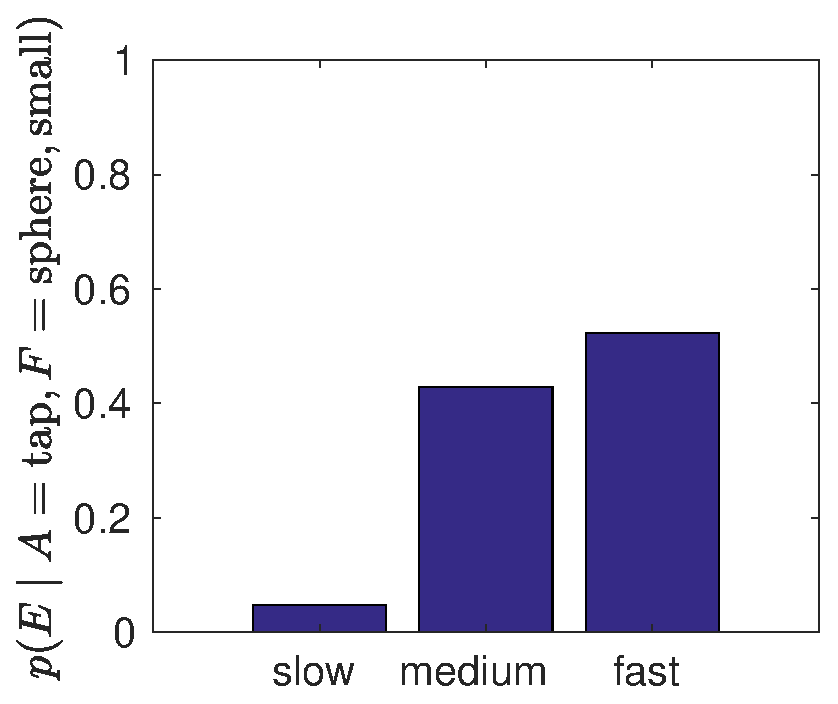
\includegraphics[width=0.45\linewidth]{effectpred_sphere.eps} \label{fig:effect_pred:sphere} } \quad
    %
    \subfloat[][Prediction of the movement effect on a big box.]
    { 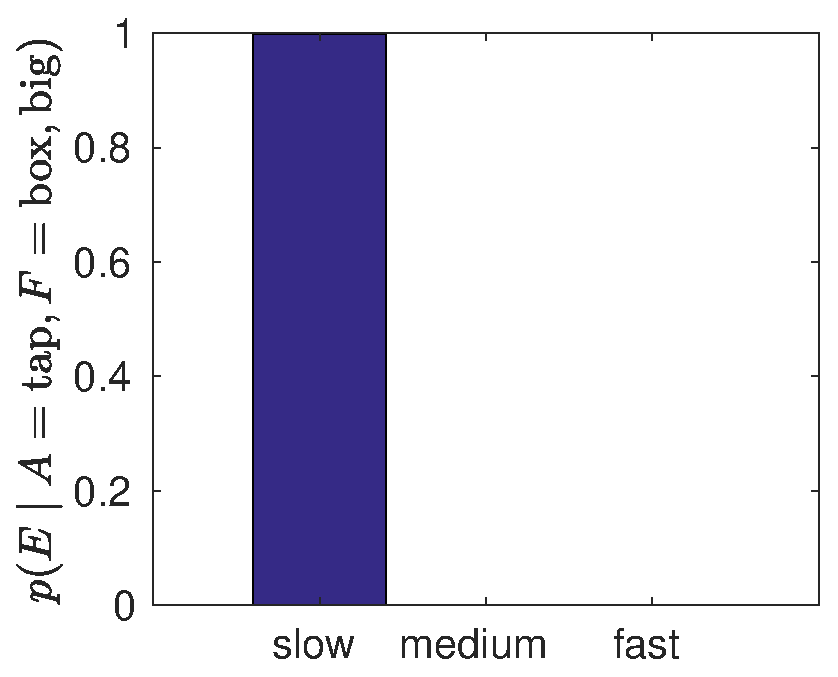
\includegraphics[width=0.45\linewidth]{effectpred_box.eps} \label{fig:effect_pred:box} }
    \caption{Object velocity predictions, given prior information~(from Gesture \acp{HMM}) that the human user performs a tapping action.}
    \label{fig:effect_pred}
\end{figure}

\section{Experimental Results}

We present preliminary examples of two types of results: predictions over the effects of actions onto environment objects, and predictions over the associated word descriptions in the presence or absence of an action prior. In this section, we assume that the Gesture \acp{HMM} provide the discrete value of the recognized action performed by a human agent~(\ie, we enforce a hard decision over the observed action, referring to the possible combination strategies listed in Sec.~\ref{sec:combination}).

\subsection{Effect Prediction}

From our combined model of words, affordances and observed actions, we report the inferred posterior value of the Object Velocity effect, given prior information about the action~(provided by the Gesture \acp{HMM}) and also about object features~(Shape and Size). Fig.~\ref{fig:effect_pred} shows the computed predictions in two cases. Fig.~\ref{fig:effect_pred:sphere} shows the anticipated object velocity when the human user performs the tapping action onto a small spherical object, whereas Fig.~\ref{fig:effect_pred:box} displays it when the target object is a big box. Indeed, given the same observed action prior~(lateral tap on the object), the expected movement is very different depending on the physical properties of the target object.
% presently, the BN is agnostic to which agent is performing an Action. correspondence problem, future work?

\begin{figure}
\centering
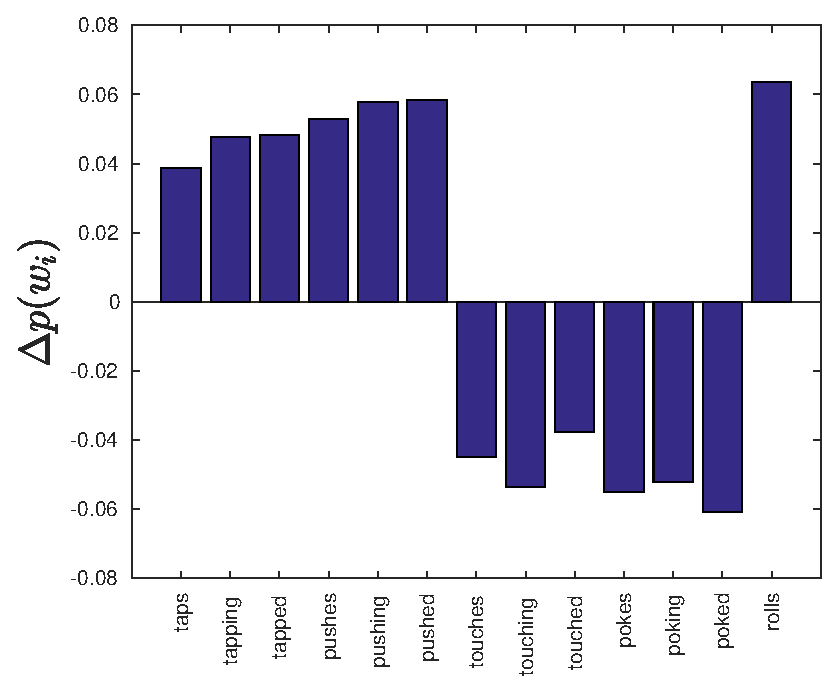
\includegraphics[width=0.9\columnwidth]{partialfig.eps}
\caption{Variation of word occurrence probabilities when we add the tap action evidence~(obtained from the Gesture \acp{HMM}) to the initial evidence about object features and effects. We have omitted words for which no significant variation was observed.}
\label{fig:probdiff}
\end{figure}

\subsection{Prediction of Words}

In this experiment, we compare the associated verbal description obtained by the \acl{BN} in the absence of an action prior, with the ones obtained in the presence of one. In particular, we compare the probability of word occurrence in these two situations:
\begin{enumerate}
\item when the robot prior knowledge~(evidence in the \ac{BN}) includes information about object features and effects only: \emph{Size=big, Shape=sphere, ObjVel=fast};

\item when the robot prior knowledge includes, in addition to the above, evidence about the action as observed from the Gestures \acp{HMM}, in particular \emph{Action=tap}.
\end{enumerate}

Fig.~\ref{fig:probdiff} shows the variation in word occurrence probabilities between the two cases,
\begin{equation} \label{eq:delta_word_prob}
\begin{split}
%\begin{align}
  \Delta p(w_i) = p(w_i \mid \text{Size=big, Shape=sphere, ObjVel=fast}) +\\
                - p(w_i \mid \text{Size=big, Shape=sphere, ObjVel=fast, Action=tap} ),
%\end{align}
\end{split}
\end{equation}
where we have omitted words for which no significant variation was observed in this case. We can interpret the difference in the predictions as follows:
\begin{itemize}
\item as expected, the probabilities of words related to tapping and pushing increase when a tapping action evidence from the Gestures \acp{HMM} is introduced; conversely, the probabilities of other action words~(touching and poking) decreases;

\item interestingly, the probability of the word \emph{rolling}~(which is an effect of an action onto an object) also increases when the tapping action evidence is entered. Even though the initial evidence of case~$1$ already included some effect information~(the velocity of the object), it is only now, when the robot perceives that the physical action was a tap, that the event rolling is associated.
\end{itemize}

%We compare the \ac{BN} predictive power in terms of word nodes, with and without the Action prior information provided by the Gesture \acp{HMM}. In other words, we compare~$p(W \mid A, E, F)$ with~$p(W \mid E, F)$.

%TODO work in progress, looking for a combination of E,F which makes the result significant


%%%%%%%%%%%%%%%%%%%%%%%%%%%%%%%%%%%%%%%%%%%%%%%%%%%%%%%%%%%%%%%%%%%%%%%%%%%%%%%%
%!TEX encoding = UTF-8 Unicode

\section{Conclusions and Future Work}

blah


%%%%%%%%%%%%%%%%%%%%%%%%%%%%%%%%%%%%%%%%%%%%%%%%%%%%%%%%%%%%%%%%%%%%%%%%%%%%%%%%
\section{Acknowledgements}
This research was partly supported by the CHIST-ERA project IGLU and by the FCT project~UID/EEA/50009/2013.
We thank Konstantinos~Theofilis for his software and help permitting the acquisition of human hand coordinates in \hri{} scenarios with the iCub robot.%~(\url{http://wiki.icub.org/wiki/OpenNI2}). % TODO uncomment

%%%%%%%%%%%%%%%%%%%%%%%%%%%%%%%%%%%%%%%%%%%%%%%%%%%%%%%%%%%%%%%%%%%%%%%%%%%%%%%%
%The reference format is the standard IEEE one. References should be numbered in order of appearance
%\newpage
%\balance
\nocite{*} % TODO remove this when article is finished
\bibliographystyle{IEEEtran}
%\bibliographystyle{IEEEtran/bibtex/IEEEtran}
\bibliography{glu2017_bibliography}

\end{document}
